\chapter{Resultados e discussão}
\label{cap:resultados-e11}

\section{Viabilidade funcional e integridade da amostra}

As 30 rodadas previstas foram concluídas, com dez por cenário. Todas as 30.000 requisições registraram HTTP 200 e identificadores únicos. Em cada rodada, a auditoria conciliou 874 mudanças de atributo, 126 operações sem alteração, 500 notificações de condição e 250 efeitos com os registros do cliente, os logs de serviço e o oráculo regenerado. A Tabela~\ref{tab:resultado-funcional} apresenta as contagens agregadas por cenário.

\begin{table}[htbp]
\centering\small
\caption{Resultados funcionais auditados por cenário.}
\label{tab:resultado-funcional}
\begin{tabular}{@{}lrrrrr@{}}
\toprule
Cenário & Rodadas & HTTP 200 & Mudanças & Condições & Efeitos \\
\midrule
C2 & 10 & 10.000 & 8.740 & 5.000 & 2.500 \\
C3 & 10 & 10.000 & 8.740 & 5.000 & 2.500 \\
C4 & 10 & 10.000 & 8.740 & 5.000 & 2.500 \\
\midrule
Total & 30 & 30.000 & 26.220 & 15.000 & 7.500 \\
\bottomrule
\end{tabular}
\fonte{Dados auditados da campanha principal}
\end{table}

As identidades das três instâncias de serviço foram preservadas durante os lotes e os registros indicaram zero reinícios. A auditoria também verificou a correspondência entre mensagens e efeitos, e não apenas a igualdade das contagens. Essa diferença é importante: duas execuções podem produzir a mesma quantidade de efeitos e ainda divergir na ordem ou nas entradas que os causaram. A conciliação com o oráculo e com as relações causais sustenta a preservação funcional nos casos exercitados.

A execução em C3 demonstra que a aplicação adaptada funcionou com seus três serviços em Pods distintos no mesmo nó virtual. C4 amplia essa evidência para o percurso entre dois nós kind. O resultado responde à questão de viabilidade da implantação delimitada no trabalho, sem estender a conclusão a outros conjuntos de regras, execução concorrente ou falhas com perda de estado.

\section{Tempo de lote e vazão}

A Tabela~\ref{tab:e11-resumo} separa mediana, quartis e extremos em colunas para facilitar a leitura. Cada linha sintetiza dez rodadas. Os tempos medianos de lote foram 18,09 s em C2, 18,35 s em C3 e 19,03 s em C4. As vazões medianas correspondentes foram 55,29, 54,49 e 52,56 requisições por segundo.

\begin{table}[htbp]
\centering\small
\caption{Duração, vazão e RTT típico entre as dez rodadas de cada cenário.}
\label{tab:e11-resumo}
\setlength{\tabcolsep}{4pt}
\begin{tabular}{@{}llrrrrr@{}}
\toprule
Métrica & Cenário & Mediana & Q1 & Q3 & Mínimo & Máximo \\
\midrule
Lote (s) & C2 & 18,09 & 17,86 & 18,28 & 17,61 & 18,94 \\
Lote (s) & C3 & 18,35 & 18,19 & 18,74 & 17,59 & 20,37 \\
Lote (s) & C4 & 19,03 & 18,75 & 20,60 & 18,29 & 27,52 \\
Vazão (req/s) & C2 & 55,29 & 54,71 & 55,98 & 52,79 & 56,80 \\
Vazão (req/s) & C3 & 54,49 & 53,36 & 54,97 & 49,09 & 56,85 \\
Vazão (req/s) & C4 & 52,56 & 48,63 & 53,33 & 36,34 & 54,67 \\
RTT mediano (ms) & C2 & 17,64 & 17,61 & 17,66 & 17,57 & 18,12 \\
RTT mediano (ms) & C3 & 18,08 & 18,02 & 18,11 & 17,95 & 18,96 \\
RTT mediano (ms) & C4 & 18,31 & 18,28 & 19,00 & 18,22 & 23,30 \\
\bottomrule

\end{tabular}
\fonte{Dados da campanha principal}
\end{table}

A vazão da Equação~\ref{eq:tempo-vazao} usa a mesma duração do lote e não fornece uma segunda confirmação independente de vantagem ou desvantagem. Como a carga é serial, o cliente limita a emissão ao término de cada resposta. Os valores observados não devem ser interpretados como taxa máxima de atendimento nem como resultado de um teste de saturação.

A Figura~\ref{fig:e11-blocos} e a Tabela~\ref{tab:e11-blocos} preservam a estrutura dos blocos. C4 apresentou seu maior tempo em B01, com 27,52 s. A exibição de todos os valores permite observar que as diferenças não foram constantes ao longo da campanha.

\begin{figure}[htbp]
\centering
\caption{Tempo de lote observado em cada bloco da campanha principal.}
\label{fig:e11-blocos}
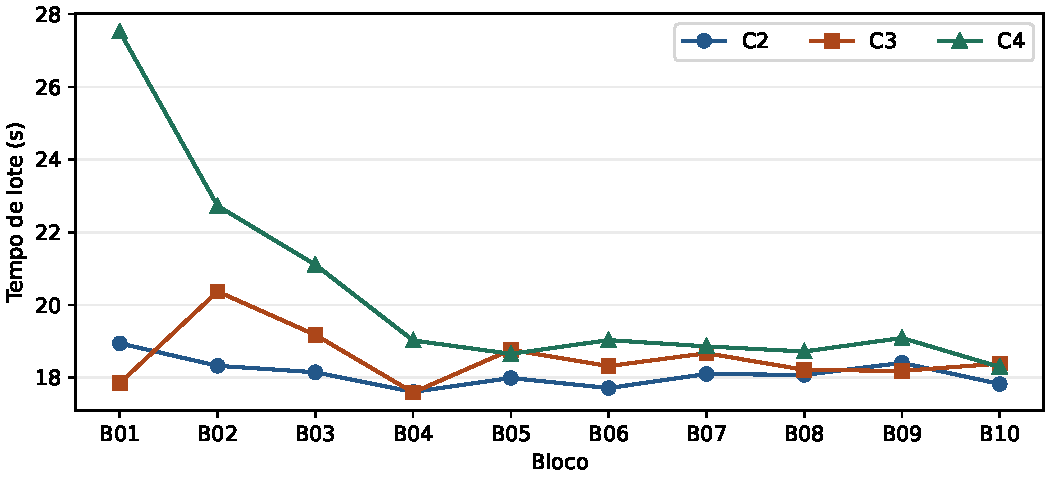
\includegraphics[width=\linewidth]{e11-m01-tempos-por-bloco.pdf}
\fonte{}
\end{figure}

\begin{table}[htbp]
\centering\small
\caption{Ordem dos cenários e duração de cada lote, em segundos.}
\label{tab:e11-blocos}
\begin{tabular}{@{}llrrr@{}}
\toprule
Bloco & Ordem de execução & C2 & C3 & C4 \\
\midrule
B01 & C2/C3/C4 & 18,94 & 17,85 & 27,52 \\
B02 & C3/C4/C2 & 18,32 & 20,37 & 22,72 \\
B03 & C4/C2/C3 & 18,15 & 19,17 & 21,11 \\
B04 & C4/C3/C2 & 17,61 & 17,59 & 19,02 \\
B05 & C3/C2/C4 & 17,99 & 18,76 & 18,65 \\
B06 & C2/C4/C3 & 17,71 & 18,32 & 19,03 \\
B07 & C2/C3/C4 & 18,10 & 18,67 & 18,86 \\
B08 & C3/C4/C2 & 18,07 & 18,21 & 18,72 \\
B09 & C4/C2/C3 & 18,40 & 18,18 & 19,09 \\
B10 & C4/C3/C2 & 17,82 & 18,39 & 18,29 \\
\bottomrule

\end{tabular}
\fonte{Dados da campanha principal}
\end{table}

Os maiores contrastes envolvendo C4 ocorreram nos primeiros blocos. O desenho não permite identificar sua causa apenas pelo formato das curvas: aquecimento de componentes da plataforma, competição de recursos e posição temporal são explicações possíveis, mas não foram isoladas por intervenções específicas. B01 foi mantido conforme o planejamento, incluindo o registro da revisão distinta na execução de B01/C2. Retirá-lo depois de observar o tempo elevado reduziria artificialmente a variabilidade apresentada.

\section{Latência típica e caudas da distribuição}

A Tabela~\ref{tab:e11-cauda} reúne os percentis e a amplitude dos RTTs. Cada p95 ou p99 foi calculado dentro de uma rodada; as colunas sintetizam depois os dez valores obtidos. Assim, as linhas não descrevem uma distribuição formada pela mistura de todas as requisições de um cenário.

\begin{table}[htbp]
\centering\small
\caption{Caudas e amplitude do RTT, em milissegundos, entre as dez rodadas.}
\label{tab:e11-cauda}
\setlength{\tabcolsep}{4pt}
\begin{tabular}{@{}llrrrrr@{}}
\toprule
Métrica & Cenário & Mediana & Q1 & Q3 & Mínimo & Máximo \\
\midrule
RTT p95 (ms) & C2 & 47,01 & 46,26 & 48,45 & 44,83 & 50,00 \\
RTT p95 (ms) & C3 & 45,17 & 42,82 & 48,04 & 38,66 & 50,14 \\
RTT p95 (ms) & C4 & 47,24 & 45,37 & 49,90 & 44,34 & 65,87 \\
RTT p99 (ms) & C2 & 82,94 & 80,00 & 87,17 & 76,21 & 90,02 \\
RTT p99 (ms) & C3 & 85,77 & 84,63 & 87,90 & 82,43 & 96,67 \\
RTT p99 (ms) & C4 & 88,08 & 84,76 & 99,60 & 81,61 & 131,72 \\
Amplitude RTT (ms) & C2 & 123,51 & 121,99 & 134,62 & 115,99 & 189,11 \\
Amplitude RTT (ms) & C3 & 150,07 & 138,09 & 167,88 & 118,06 & 246,76 \\
Amplitude RTT (ms) & C4 & 175,78 & 150,35 & 196,10 & 129,28 & 338,75 \\
\bottomrule

\end{tabular}
\fonte{Dados da campanha principal}
\end{table}

A mediana entre rodadas do p99 foi 82,94 ms em C2, 85,77 ms em C3 e 88,08 ms em C4. Para o p95, os intervalos observados se sobrepuseram e C3 apresentou a menor mediana entre rodadas. Portanto, a ordenação dos cenários depende da métrica utilizada: um menor p95 não significa necessariamente menor duração total ou menor p99.

\begin{figure}[htbp]
\centering
\caption{Percentis 95 e 99 do RTT por bloco da campanha principal.}
\label{fig:e11-cauda}
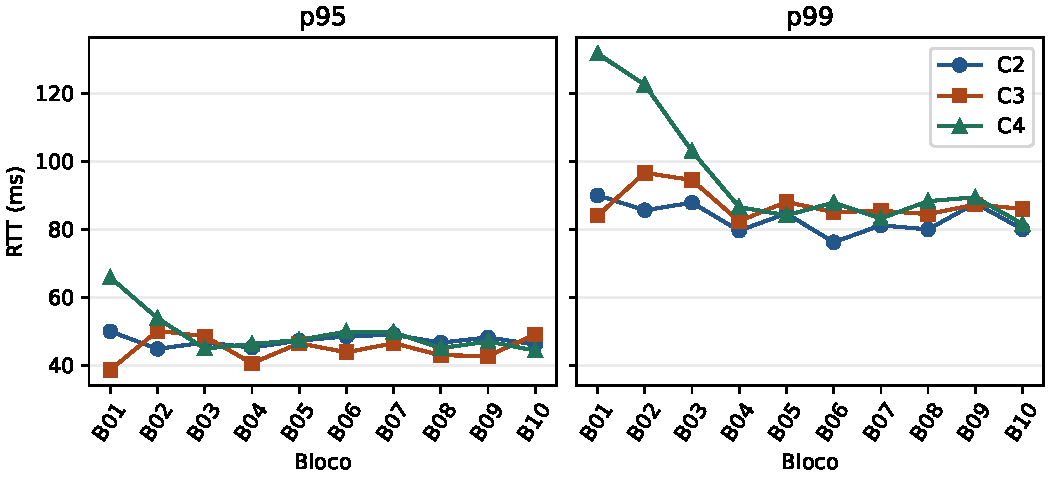
\includegraphics[width=\linewidth]{e11-m01-cauda-rtt.pdf}
\fonte{}
\end{figure}

O RTT inclui o processamento e o retorno síncrono do caminho efetivamente percorrido. Como a carga combina operações sem mudança, mudanças sem transição e mudanças com efeito, há percursos distintos dentro do mesmo lote. A análise apresentada descreve a composição fixa da carga. Não foram estimados efeitos causais separados por tipo de percurso nem uma latência de rede obtida por subtração de relógios entre serviços.

O p99 também depende de uma porção pequena das 1.000 observações ordenadas de cada rodada. Sua apresentação é útil para tornar visíveis respostas mais lentas, mas não estabelece um compromisso de nível de serviço para produção. A amplitude mostra a distância entre extremos e, por construção, pode ser influenciada por poucas observações.

\section{Comparação pareada por bloco}

A Tabela~\ref{tab:e11-diferencas} mostra as diferenças de duração em cada bloco, e a Tabela~\ref{tab:e11-pares} sintetiza diferenças e razões. Essa separação evita reunir tempos, diferenças e razões em uma única célula. Nas razões, o cenário à esquerda é o numerador; valores acima de um indicam maior duração.

\begin{table}[htbp]
\centering\small
\caption{Diferenças pareadas de duração, em segundos.}
\label{tab:e11-diferencas}
\begin{tabular}{@{}lrrr@{}}
\toprule
Bloco & C3 menos C2 & C4 menos C2 & C4 menos C3 \\
\midrule
B01 & -1,09 & 8,58 & 9,67 \\
B02 & 2,04 & 4,40 & 2,36 \\
B03 & 1,03 & 2,96 & 1,93 \\
B04 & -0,02 & 1,42 & 1,43 \\
B05 & 0,77 & 0,66 & -0,11 \\
B06 & 0,61 & 1,32 & 0,71 \\
B07 & 0,57 & 0,76 & 0,19 \\
B08 & 0,14 & 0,64 & 0,50 \\
B09 & -0,22 & 0,69 & 0,91 \\
B10 & 0,56 & 0,47 & -0,09 \\
\bottomrule

\end{tabular}
\fonte{Dados da campanha principal}
\end{table}

\begin{table}[htbp]
\centering\small
\caption{Síntese dos contrastes pareados entre as dez rodadas.}
\label{tab:e11-pares}
\setlength{\tabcolsep}{4pt}
\begin{tabular}{@{}llrrrrr@{}}
\toprule
Contraste & Medida & Mediana & Q1 & Q3 & Mínimo & Máximo \\
\midrule
C3/C2 & Diferença (s) & 0,57 & 0,02 & 0,73 & -1,09 & 2,04 \\
C3/C2 & Razão & 1,032 & 1,001 & 1,041 & 0,942 & 1,112 \\
C4/C2 & Diferença (s) & 1,04 & 0,67 & 2,57 & 0,47 & 8,58 \\
C4/C2 & Razão & 1,058 & 1,037 & 1,142 & 1,026 & 1,453 \\
C4/C3 & Diferença (s) & 0,81 & 0,27 & 1,81 & -0,11 & 9,67 \\
C4/C3 & Razão & 1,044 & 1,014 & 1,096 & 0,994 & 1,542 \\
\bottomrule

\end{tabular}
\fonte{Dados da campanha principal}
\end{table}

A diferença mediana C3 menos C2 foi 0,57 s, com C3 mais lento em sete blocos. C4 levou mais tempo que C2 nos dez blocos, com diferença mediana de 1,04 s e razão mediana de aproximadamente 1,06. Em relação a C3, C4 levou mais tempo em oito blocos, com diferença mediana de 0,81 s. A Figura~\ref{fig:e11-contrastes} permite visualizar a direção e a magnitude dos contrastes.

\begin{figure}[htbp]
\centering
\caption{Diferenças de duração por bloco; valores positivos indicam maior tempo do primeiro cenário.}
\label{fig:e11-contrastes}
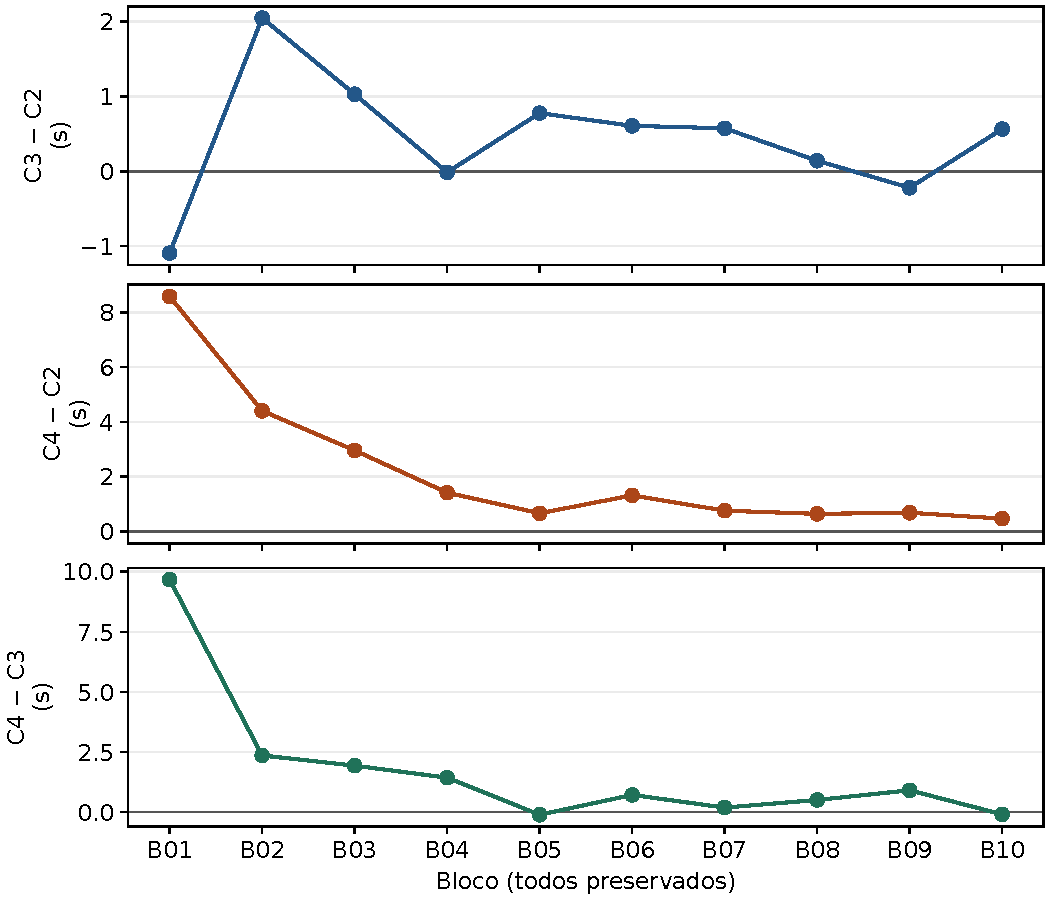
\includegraphics[width=.96\linewidth]{e11-m01-contrastes-pareados.pdf}
\fonte{}
\end{figure}

Esses valores são medianas das comparações dentro de cada bloco. Por exemplo, a diferença entre as medianas de C3 e C2, arredondadas na Tabela~\ref{tab:e11-resumo}, é 0,26 s, enquanto a mediana das diferenças pareadas é 0,57 s. Não há contradição: os estimadores usam operações distintas. O pareamento mantém a associação planejada entre as três execuções de um bloco.

A regularidade da direção C4 maior que C2 é um resultado descritivo da amostra. Ela não estabelece significância estatística nem um percentual universal de custo. Também não permite decompor a diferença total em parcelas independentes de Docker, Kubernetes e transporte: as camadas interagem e o posicionamento do avaliador difere entre as configurações.

\section{Ameaças à validade e alcance dos resultados}

Quanto à validade interna, os blocos, a carga fixa, a imagem conferida e o estado inicial novo reduzem fontes de variação identificadas no procedimento. Permanecem possíveis interferências do host, das camadas de virtualização e da ordem temporal. O posicionamento no control-plane em C4 também pode interagir com serviços de controle. A variação entre execuções e a ordem de ensaios são riscos reconhecidos em estudos de desempenho \cite{maricq2018taming,duplyakin2023ordering}; este trabalho os torna visíveis, sem afirmar que foram eliminados.

Quanto à validade de construto, o tempo do lote caracteriza o caminho completo da aplicação e do cliente, sob os limites escolhidos. Ele não representa CPU utilizada, energia ou custo puro de rede. Da mesma forma, receber HTTP 200 não seria suficiente para demonstrar preservação funcional; por isso, a auditoria também utilizou o oráculo, as sequências e os efeitos. As cotas de CPU e memória são condições do ensaio, não métricas de consumo.

Quanto à validade externa, a investigação cobre uma prova de conceito, uma condição lógica, uma carga de 1.000 operações seriais e um host físico. Dois nós kind não equivalem a dois computadores independentes. Os resultados não caracterizam processamento real de vídeo, escala horizontal, operação multiusuário, tolerância à perda de nós ou capacidade máxima.

Quanto à conclusão estatística, foram preservadas dez rodadas por cenário e a análise permaneceu descritiva. Não se tratou cada requisição como réplica independente, não se excluíram blocos lentos e não se afirmou equivalência pela proximidade de medianas. Uma campanha futura com objetivo inferencial deverá definir estimador, precisão e número de repetições antes da coleta.

A leitura conjunta permite reconhecer dois resultados complementares: a cadeia adaptada preservou o comportamento funcional para as entradas cobertas, e sua duração variou entre as configurações. A viabilidade de implantação foi demonstrada nesse recorte; a vantagem de desempenho, o consumo de recursos e a escalabilidade permanecem perguntas distintas.
